\chapter{The Selfish Miner \small{\textsf{DRAFT}}}

\section{Recap of Chain Virtues}
There are 3 chain virtues that are relevant to our study:

\begin{enumerate}
    \item Common prefix with parameter $k$
    \item Chain quality with parameter $\mu$
    \item Chain growth with parameter $\tau$
\end{enumerate}


Common prefix has implications for the safety of transactions on chain. Meanwhile chain quality and chain growth affect the liveness of transactions (which refers to how much time it takes for a transaction to be confirmed after it is sent to the network).
% These are also interrelated. Chain quality implies liveness because a  transaction will be validated faster if there are more honest nodes.

\subsection{Common Prefix}

Two or more chains have a common prefix of $k$ if and only if the chains agree on all blocks except the last $k$ blocks at the end of the chains.
Chains adopted by different honest nodes satisfy the common prefix property.
The probability of violation of this property decreases exponentially as $k$ increases. The greater $k$ is, the more ``forgiving" the common prefix property is, and the longer one waits to confirm a transaction.
Common prefix property implies safety of the ledger.

\subsection{Chain Quality}
The chain adopted by any honest node contains at least $\mu$ fraction of blocks mined by honest nodes.
% (ignoring temporary forks for counting purposes). These temporary forks are not necessarily problems because they will occur even in fully honest chains.

The number of blocks mined by honest nodes in a chain is important because adoption of a chain by an honest node means it is valid (there are no double spends), but there could be a censorship attack (there are no honestly mined blocks in the chain).
This property is required for liveness as adversarially mined blocks may not contain any transactions.

\subsection{Chain Growth}
The chain adopted by an honest node grows at a rate of $\tau$ blocks per unit time. This has ramifications for how fast transactions are included in the blockchain, and hence the liveness too.
\section{Censorship Attack}
Many chain attacks fall under the umbrella of a Nakamoto race, where honest parties and the adversary race to extend the length of their respective chains. Here, we will see another kind of attack. We started with the Honest Majority Assumption (henceforth HMA) which means that honest parties have more compute power than the adversary. We will look at a censorship attack that can be carried out by the adversary when she has majority compute power.

In a censorship attack, the adversary tries to prevent a certain transaction from being confirmed. The basic idea is that when she sees a transaction $\mathsf{tx}$ in a certain block, she mines at the previous block to prevent that transaction being included in the chain.
Since the adversary has majority, she can always win the Nakamoto race and therefore replace every honest block from the longest chain.
Therefore, the transaction never enters the longest chain.
This attack breaks chain quality.
The mechanism is illustrated below.


 \begin{figure}[h!]

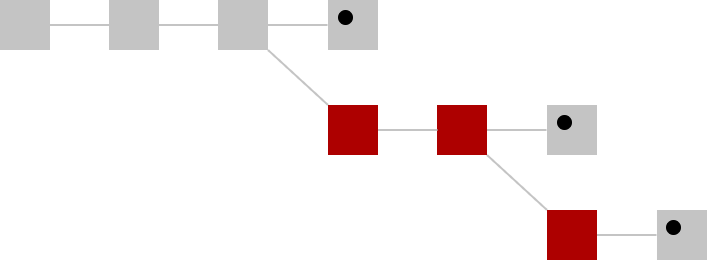
\includegraphics[scale=0.5]{figures/censorship.png}
 \caption{Depiction of a censorship attack. Grey blocks are mined by honest miners. Red blocks are valid blocks mined by the adversary. The black dot represents the transaction $\mathsf{tx}$ that the adversary is trying to censor. }
\end{figure}

\section{Attacks Under Dishonest Majority}
When honest majority holds, we have seen that the blockchain satisfies common prefix, chain quality and chain growth.
If the adversary has majority of the computing power for some time, she can break common prefix (recall the Nakamoto race attack from the previous lecture). The adversary can also break chain quality (see the censorship attack above).
However, chain growth is not broken, although it may be slowed down (i.e. the parameter $\tau$ may be reduced), because honest nodes continue to produce blocks on their longest chain.

A majority adversary can revert a transaction (by breaking common prefix). The adversary can also censor transactions (by breaking chain quality).
As a consequence, the adversary can break safety or liveness of the ledger.
However, the adversary cannot spend coins owned by an honest party because she cannot generate valid transactions for such a signature.
The adversary also cannot create more money than what is allowed by the macroeconomic policy, because such blocks would not be accepted by the honest nodes.

\section{Healing From Attacks}
Assume there is a temporary adversarial majority of compute power (TAM). Then the HMA is not respected during some time period $\delta$, and then it is respected again.
During the period of TAM, safety and liveness may not hold. The adversary can double spend and can carry out censorship attacks, violating properties like common prefix and chain quality.

After the period of TAM, when HMA is respected again, liveness heals because chain quality is recovered. Chain quality recovers because when HMA is respected, the honest parties will win the Nakamoto race and there will eventually be an honest block that includes previously censored transactions. Also, safety will heal as common prefix heals. Common Prefix recovers because of the reemergence of the HMA, and the presence of convergence opportunities means that the honest nodes will once again converge on their longest chains.

The recovery of HMA presents convergence opportunities. If convergence occurs, then any conflicting transactions which would render a block invalid (i.e. a double spend) are not included in the
honestly adopted chain
or in the mempool,
rather they are dropped.
% Chain quality heals after convergence occurrs, and honest chains are able to latch onto the same chain. Then common prefix heals when honest mining power is once more concentrated.

Since safety and liveness are not guaranteed during TAM, and it takes some time to recover safety and liveness after HMA is recovered, a user should not be using the blockchain during the TAM and a while after (if they are aware of the TAM). This is because safety and liveness cannot be recovered for coins affected during the TAM.
For example, if a car dealer delivered a car in exchange for a transaction on the blockchain during TAM, and the adversary reverted that transaction after receiving the car, that money cannot be recovered by the car dealer.


\section{Selfish Mining}
We now ask the question: Is there a lower bound on the chain quality $\mu$, and if there is, what is it? It is intuitive to guess that the lower bound is roughly the percentage of hashing power that is honest. In other words, our conjecture is that:
\begin{equation}
\label{eq:cq_conjecture}
    \mu \geq \frac{n-t}{n}
\end{equation}
We will see now that this is false. \\
Consider the selfish miner $\mathcal{A}$, who does the following:
\begin{enumerate}
    \item Adopt the longest chain
    \item Mine in secret extending the last block of the longest chain
    \item When an honest block is found:
    \begin{enumerate}
        \item If $\mathcal{A}$ has a secret block, broadcast it.
        \item Otherwise, adopt the honest tip.
    \end{enumerate}
    Then repeat from Step 2.
\end{enumerate}


Here, the adversary $\mathcal{A}$ is also a “rushing adversary”, which is one who sees honestly broadcasted messages prior to everybody else. As such, since $\mathcal{A}$ can broadcast her own block before the honest block gets to the rest of the honest miners, the honest miners will adopt $\mathcal{A}$'s block and start building the next block off of that. The honest block that $\mathcal{A}$ had originally seen is now wasted effort. If this continues, the block tree may look something like this:

\begin{figure}[h!]
\[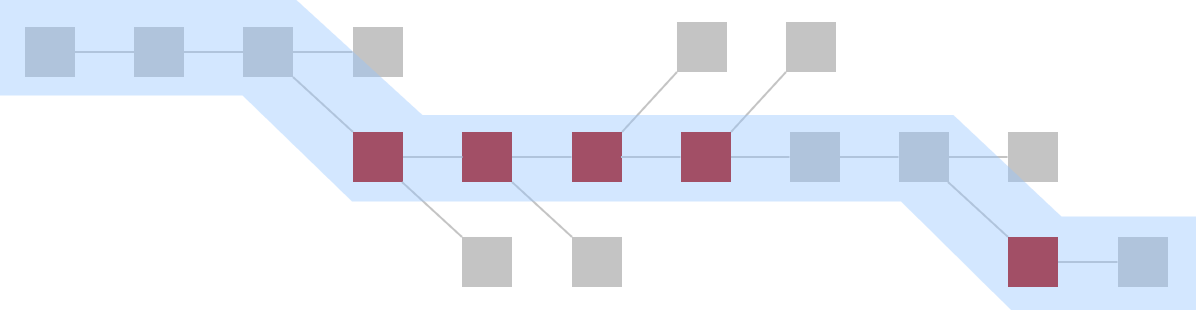
\includegraphics[scale=0.4]{figures/longestchain.png}\]
\caption{In this example, suppose that $n=17$, $t=5$ and $\frac{n-t}{n} \approx 0.71$. There are $5$ adversarial blocks and $12$ honest blocks mined which are proportional to the compute powers. In the longest chain here (highlighted in blue), there are $5$ adversarial blocks and $11$ total blocks, so we can see that $\mu \approx 0.55$. Thus, we can see that our earlier conjecture (\eqref{cq_conjecture}) is false.}
\end{figure}

Due to the wasted efforts of the honest blocks, we can start to see that $\mu$ is not necessarily equal to the fraction of honest mining power. None of the adversarial blocks are wasted in this example, but many of the honest ones are. The goal of the selfish mining attack is for every single adversarial block to be contained in the longest chain.

Below is the simulation in typescript for selfish mining. If you run it yourself, you'll see that chain quality is on average less than 0.1, even though adversarial power is 0.49.
\begin{tcolorbox}[colback=gray!30]
{\small\begin{alltt}
\begin{verbatim}
const ADVERSARIAL_POWER = 0.49
const BLOCK_LIMIT = 500
const MONTE_CARLO = 10

function simulate() {
  let honestBlocks = 1
  let adversaryHeadStart = 0
  let chainLength = 1

  while (chainLength < BLOCK_LIMIT) {
    if (Math.random() < ADVERSARIAL_POWER) {
      // adversary got a block
      ++adversaryHeadStart
    }
    else {
      // honest got a block
      if (adversaryHeadStart > 0) {
        --adversaryHeadStart
      }
      else {
        ++honestBlocks
      }
      ++chainLength
    }
  }
  return honestBlocks / BLOCK_LIMIT
}

let sumQuality = 0

for (let i = 0; i < MONTE_CARLO; ++i) {
  sumQuality += simulate()
}
console.log(sumQuality / MONTE_CARLO)
\end{verbatim}
\end{alltt}}
\end{tcolorbox}

In conclusion, an adversary does not need much mining power in order to incur heavy damage on chain quality.

\section{What Value of $T$ to Choose?}
Last class, we discussed how neither a high $T$ nor a low $T$ necessarily allows for the optimal convergence opportunity frequency. With a high $T$, blocks are produces more frequently, but they're so frequent that convergence opportunities are extremely rare. With an extremely low $T$, nearly every block is a convergence opportunity, but the blocks are so infrequent that the absolute frequency of convergence opportunities is low. So, what is the optimal $T$, you wonder? Below is the code for simulating convergence opportunity frequency with varying $T$, followed by the accompanying generated plot.
\begin{tcolorbox}[colback=gray!30]
{\small\begin{alltt}
\begin{verbatim}
import random
import matplotlib.pyplot as plt
import numpy as np

MONTE_CARLO_REPEAT = 30
TIME_INTERVAL = 100

def simulate(eta, Delta):
  convergence_opportunities = 0
  t = 0
  prev_interarrival_time = 2 * Delta
  while t < TIME_INTERVAL:
    interarrival_time = random.expovariate(1/eta)
    if interarrival_time > Delta:
      convergence_opportunities += 1
    t += interarrival_time
    prev_interarrival_time = interarrival_time
  return convergence_opportunities

def monte_carlo(eta, Delta):
  convergence_sum = 0
  for i in range(MONTE_CARLO_REPEAT):
    convergence_sum += simulate(eta, Delta)
  return convergence_sum / MONTE_CARLO_REPEAT

Delta = 1
x = []
y = []
kappa = 256
min_T_exp = 229
max_T_exp = 239
n = 10
q = 3000000
min_eta = 0.01
max_eta = 3.0
eta_step = 0.01
# eta is the expected block interarrival time
for i, eta in enumerate(np.arange(min_eta, max_eta, eta_step)):
  T = 1 / (n * q * eta)
  x.append(T)
  y.append(monte_carlo(eta, Delta))

plt.xscale('log')
plt.xlim((2**(min_T_exp - kappa), 2**(max_T_exp - kappa)))
plt.xticks(
  [2**x for x in range(min_T_exp - kappa, max_T_exp + 1 - kappa)],
  ['$2^{' + str(x) + '}$' for x in range(min_T_exp, max_T_exp + 1)]
)
plt.plot(x, y)
plt.xlabel('Mining target $T$')
plt.ylabel(f'Convergence opportunity frequency in ${TIME_INTERVAL}$ rounds')

plt.title(f'Convergence opportunities when varying the mining target $T$.
\n$\Delta = {Delta}, n = {n}, q = 3 \cdot 10^9, \kappa = {kappa}$')
plt.show()

\end{verbatim}
\end{alltt}}
\end{tcolorbox}

\begin{figure}[h!]
\[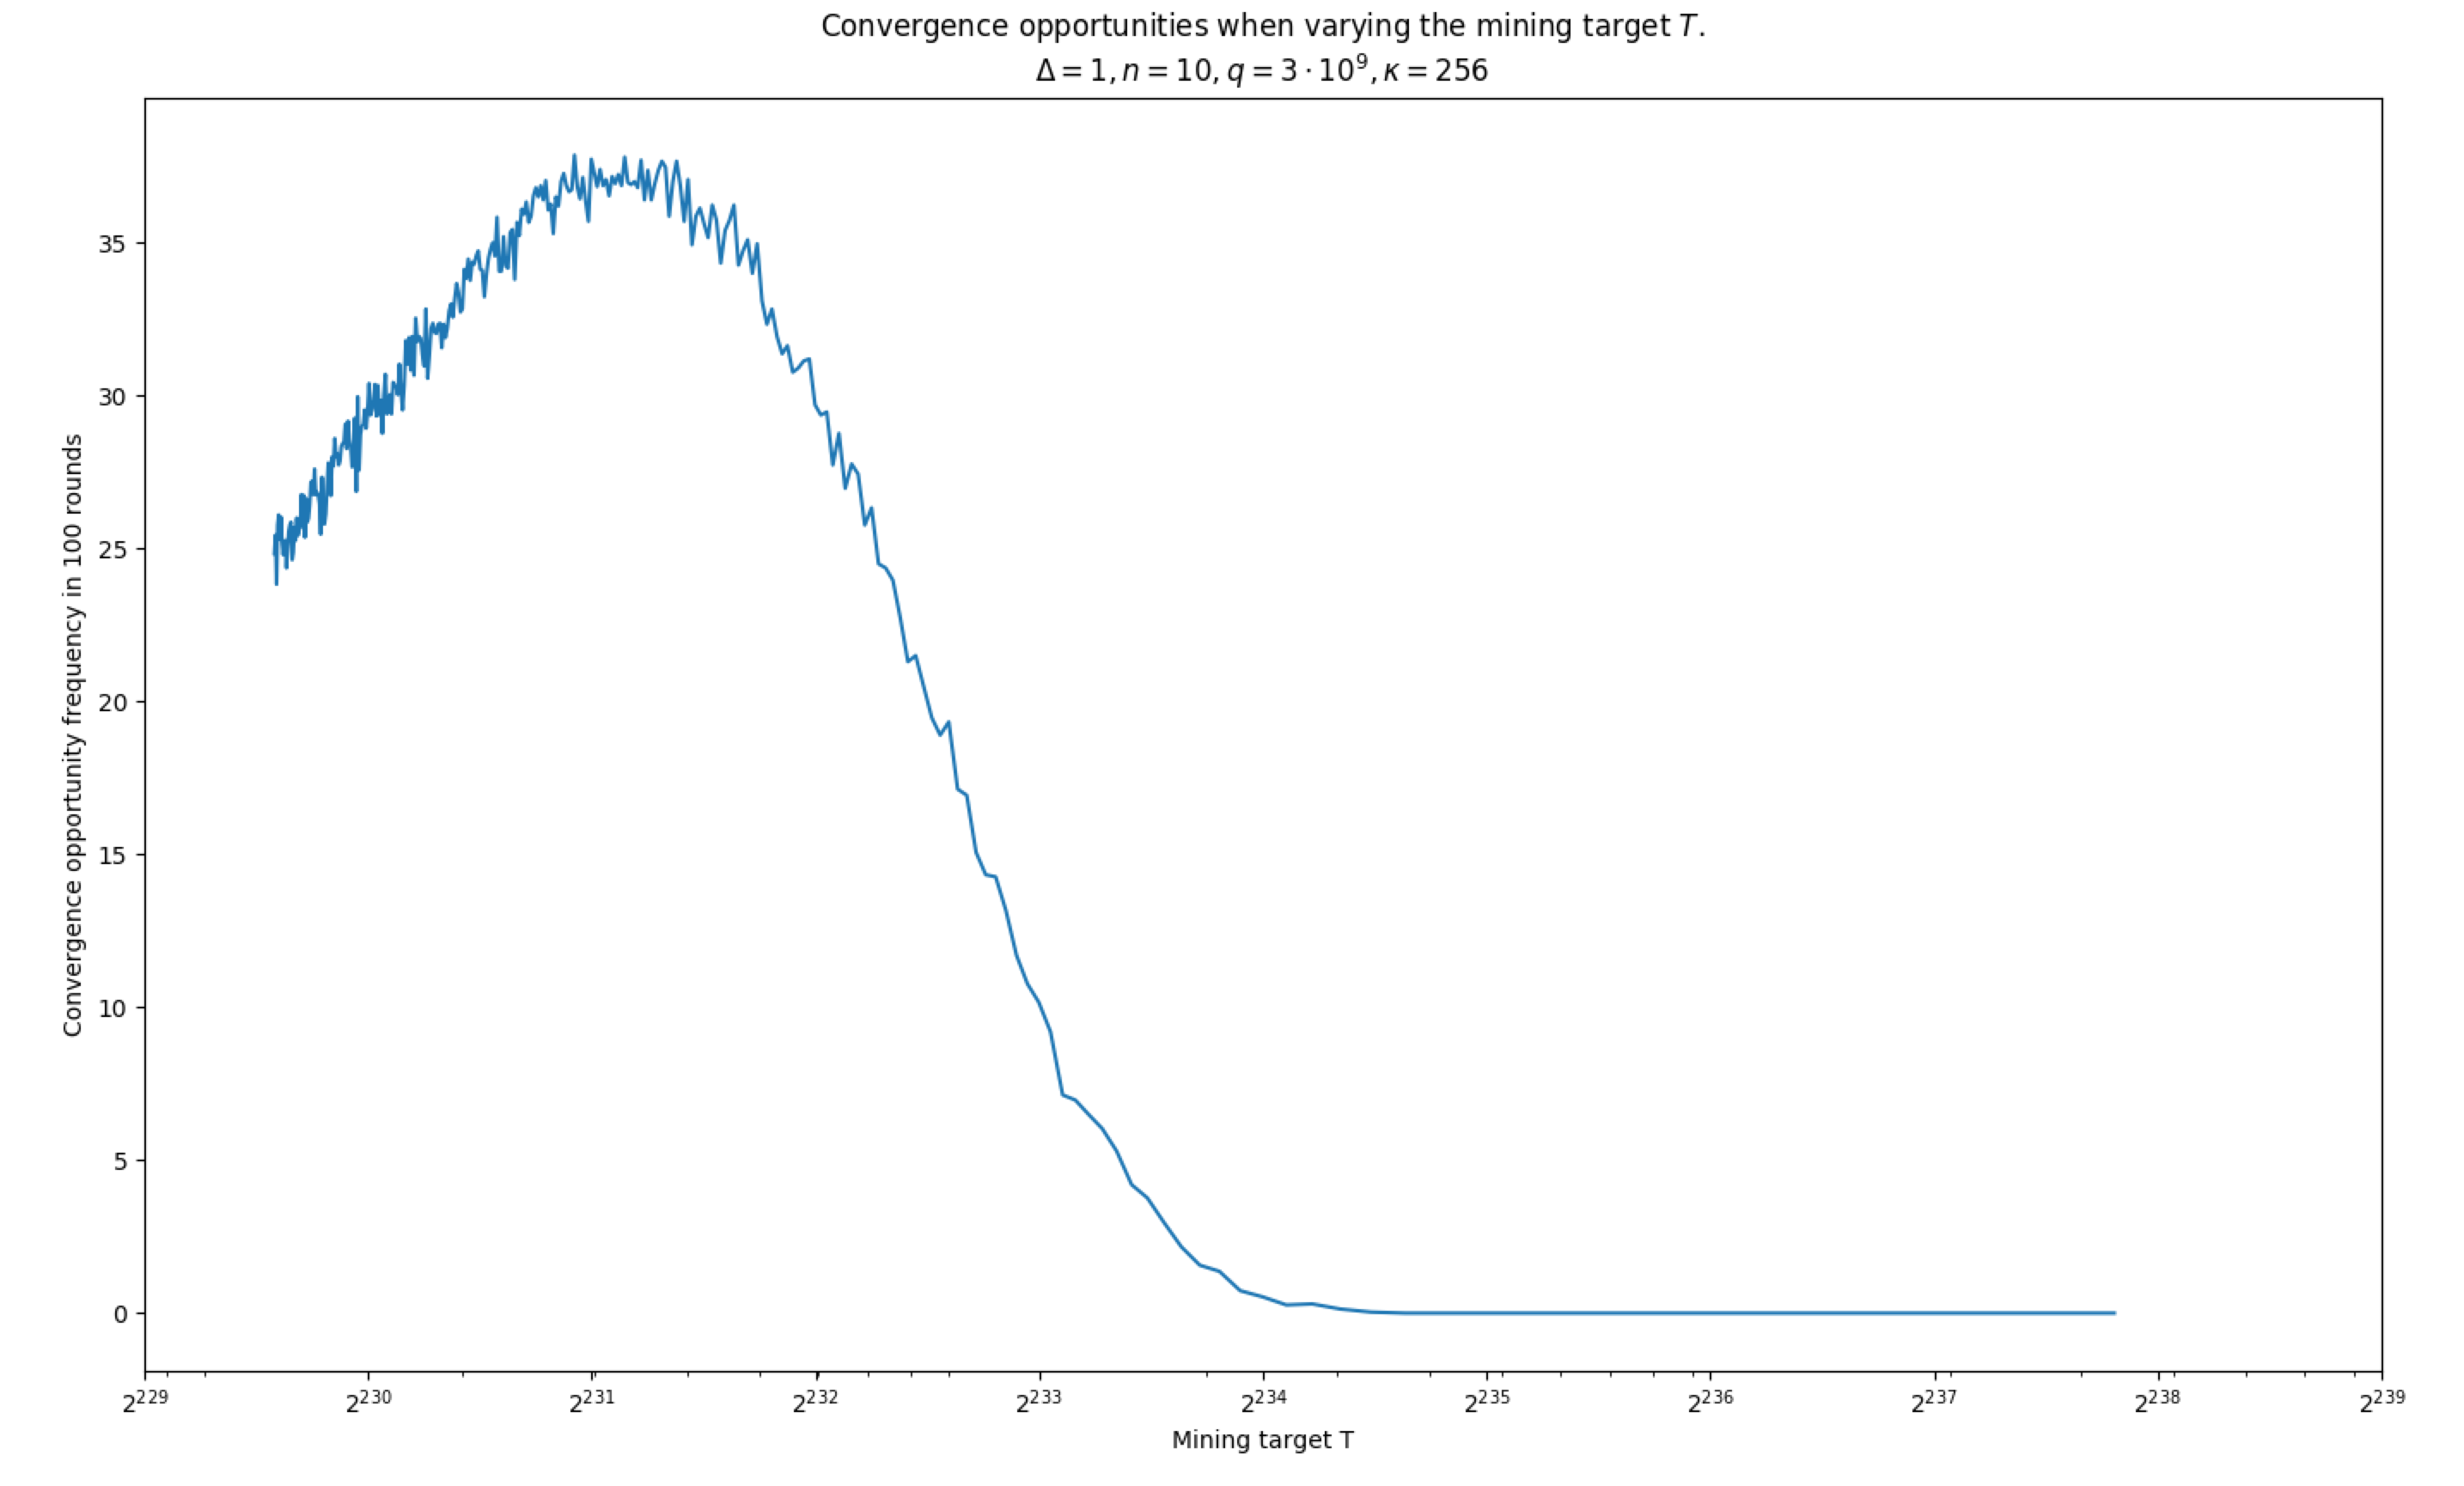
\includegraphics[scale=0.35]{figures/targetT.png}\]

\label{fig:convergence_opp_frequency}
\caption{Plot of convergence opportunity frequency versus target $T$}
\end{figure}
